\clearpage
\section{Forms}
\label{sec:builder-feature-forms}

A form is a page of questions an employee or applicant fills in, such as a leave request or a visit form. You create forms and publish their versions on the “Forms” page; a form can write its answers into a record type and can have a status and approval journey. People always work on the published version, while you edit a new draft without affecting them.

\textbf{Path and who uses it:} “Builder” → “Core” → “Forms”. Used by those with forms permission to design how requests are collected.

\begin{rcnote}[Example: Horizon]
The system administrator builds a “Branch visit request” form asking for the branch, date and purpose, and has it write the answers into “Visit requests” when Sarah Al-Khatib approves the request, so Omar Haddad fills it in without opening the record type itself. The form starts from ①.
\end{rcnote}

\begin{figure}[H]
\centering
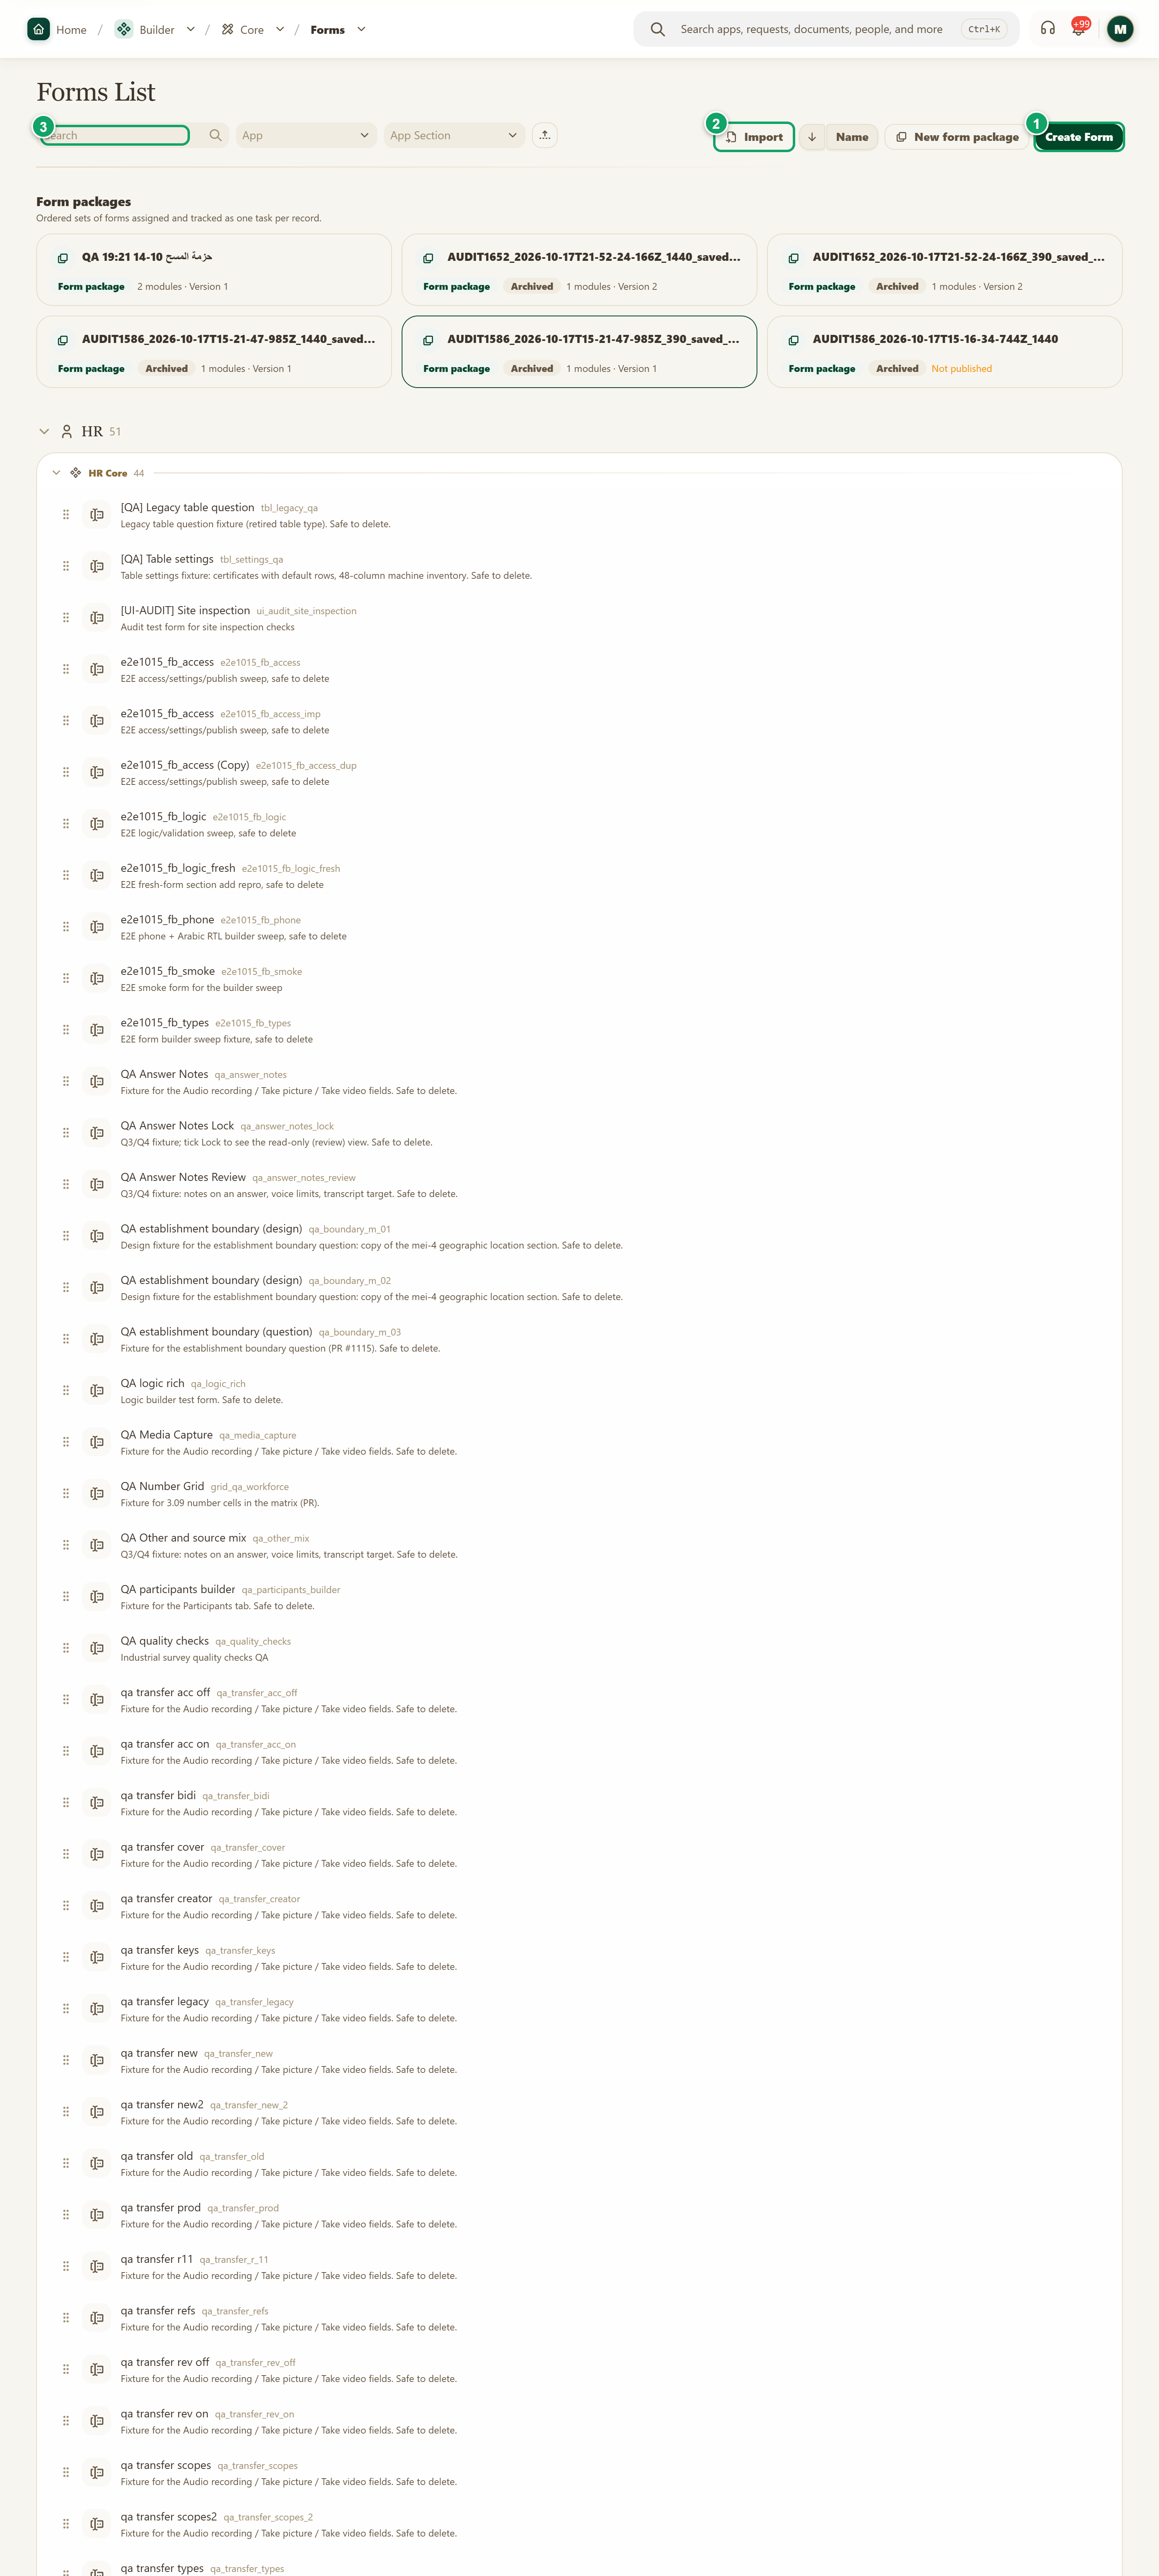
\includegraphics[width=0.95\linewidth,height=0.72\textheight,keepaspectratio]{figures/screens/ch06-forms-en.png}
\caption{The “Forms” page}
\label{fig:builder-forms-screen}
\shotnote{The page lists forms grouped by app and section, with the submission count of each. The forms shown are test forms on test2. ① “Create Form”: starts a new form. ② “Import”: creates a form from an exported file. ③ Search: finds a form by name.}
\end{figure}


\begin{table}[H]
\centering
\caption{The forms list}
\label{tab:builder-forms-list}
\begin{tabularx}{\linewidth}{R{3.6cm} Y}
\rcHeaderRow
\thh{Part} & \thh{Content and action}\\
Create Form & Asks for “Form Name”, “Form Code”, “Reference Prefix”, the app and the section, then opens the builder.\\
The list & Forms grouped by app and section, with search, sorting and submission counts, and the actions “Duplicate”, “Export form” and “Delete Form”.\\
Import & Creates a form from a previously exported file.\\
Form packages & Ordered sets of forms assigned and tracked as one task per record.\\
\end{tabularx}
\end{table}

\begin{table}[H]
\centering
\caption{The form builder's tools}
\label{tab:builder-forms-editor}
\begin{tabularx}{\linewidth}{R{3.6cm} Y}
\rcHeaderRow
\thh{Tool} & \thh{What does it do?}\\
Questions & Adds questions from groups: Text, Choice, Numbers and rating, Date and time, Place, Files \& media, and Other; plus sections, pages and text blocks.\\
Rules & Everything that shows, hides, locks, requires, calculates or checks a question, in one list.\\
Access & Who can reach each response and what they can do with it: the person who starts it, fixed people, or people chosen by the answers.\\
Journey & “Request journey”: the statuses and phases the applicant sees, the transitions between them, and approval steps.\\
Records & The records this form reads from and writes to, and when it writes: “When approved” or “When submitted”.\\
Assign & Plans that assign people to fill the form for certain records; available after the form is saved.\\
Versions and Settings & “Version history” for every version, and settings such as numbering, the PDF document and prefilled links.\\
Test form and Publish & Opens an isolated test workspace where you try the form as a member, then “Publish” makes the draft the live version.\\
\end{tabularx}
\end{table}

\begin{figure}[H]
\centering
\begin{tikzpicture}[node distance=0.5cm]
\node[stepBox] (a) {Create Form};
\node[stepBox,below=of a] (b) {Questions and rules};
\node[stepBox,below=of b] (c) {Access, journey, records};
\node[stepBox,below=of c] (d) {Test form};
\node[stepBox,below=of d] (e) {Publish};
\draw[flowsTo] (a) -- (b);
\draw[flowsTo] (b) -- (c);
\draw[flowsTo] (c) -- (d);
\draw[flowsTo] (d) -- (e);
\end{tikzpicture}
\rclegend
\caption{From idea to published form}
\label{fig:builder-forms-flow}
\shotnote{The diagram orders form building from content to behaviour: questions first, then who reaches the response and where the answers go. Testing comes before publishing because the test workspace is isolated, so it exposes mistakes without reaching anyone; publishing makes the version available to everyone who fills in the form.}
\end{figure}

\subsection{Steps and check}
\begin{enumerate}
\item Open “Forms” and press “Create Form”, then write the name, code and prefix and choose the app and section.
\item Add the questions, choosing a type that fits each answer, then add rules when needed.
\item Open “Access” to decide who sees responses, and “Records” if the answers should be written into a record type.
\item Press “Test form” and fill it in completely, then press “Publish”.
\end{enumerate}

\textbf{Check and recovery:} the message “Form published successfully” should appear, and the version should show as live in “Version history”. If the publish button turns into “Send for approval”, your organization requires publishing approval, and the form goes live after the approver agrees. If answers are not written to the record, open “Records” and check that the record type's administrator has allowed the form to write there.
